\documentclass[a4paper]{ltjsarticle}

\usepackage[margin=15mm]{geometry}

\usepackage{graphicx}

% \renewcommand{\baselinestrech}{0.8}

\begin{document}


\includegraphics[clip]{kimigayo_crop.pdf}

\vspace{-10mm}

\parindent=50pt 
君が代(きみがよはちよにやちよに)
\parindent=10pt

\vspace{10mm}



\includegraphics[clip]{schubertkomori_crop.pdf}

\vspace{-10mm}

\parindent=50pt 
シューベルトの子守唄(ねむれねむらははのむねに)
\parindent=10pt

\vspace{10mm}


\includegraphics[clip]{schubertnobara_crop.pdf}

\vspace{-10mm}

\parindent=50pt 
シューベルトの野ばら(わらべはみたりのなかのばら)
\parindent=10pt

\vspace{10mm}

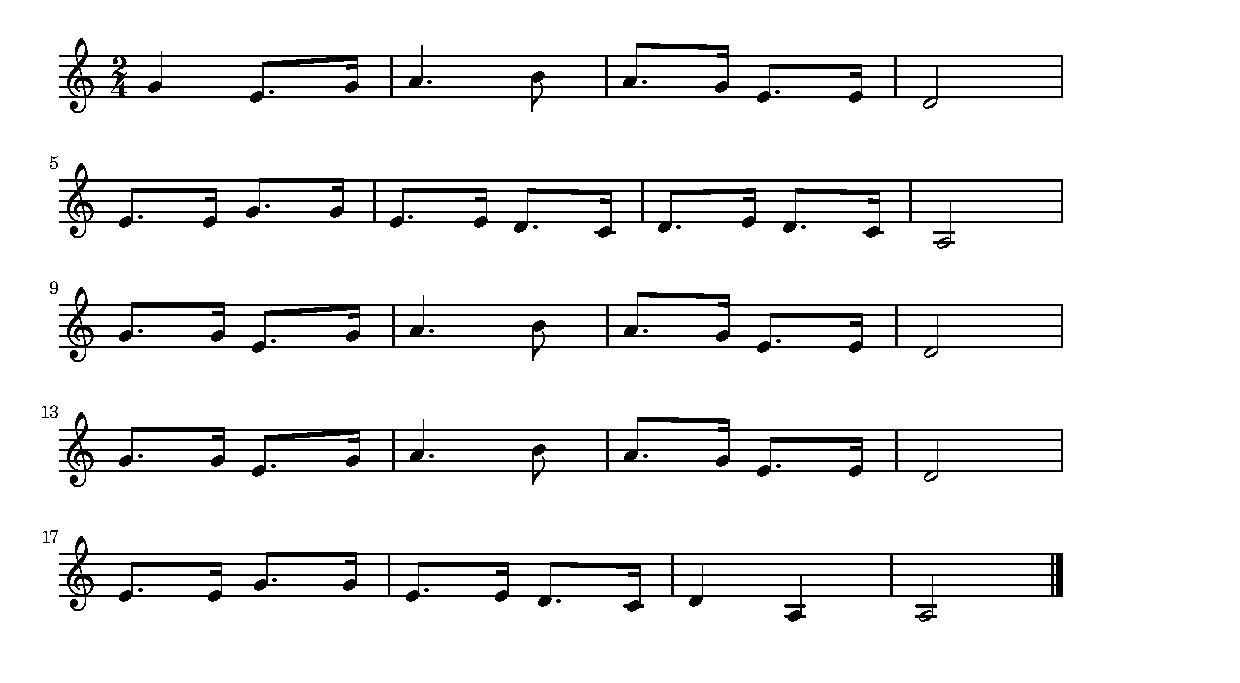
\includegraphics[clip]{yakyuken_crop.pdf}

\vspace{-10mm}

\parindent=50pt 
野球拳(やきゅうけん。やきゅうするならこういうぐあいにしやしゃんせ)
\parindent=10pt

\vspace{10mm}

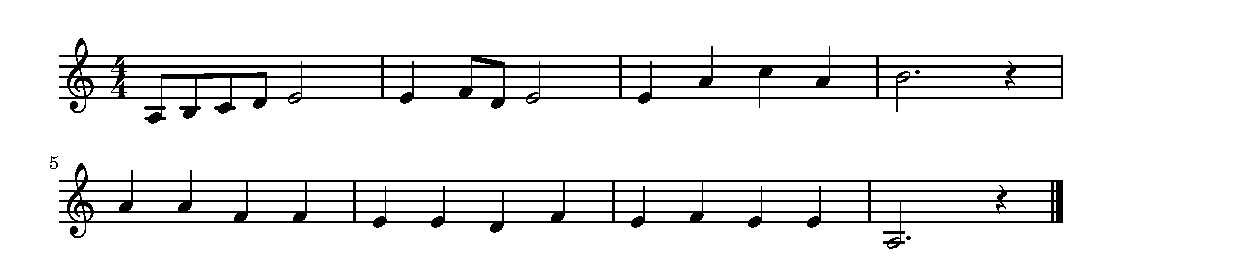
\includegraphics[clip]{akaikutsu_crop.pdf}

\vspace{-10mm}

\parindent=50pt
赤い靴(あかいくつはいてたおんなのこ)
\parindent=10pt

\vspace{10mm}

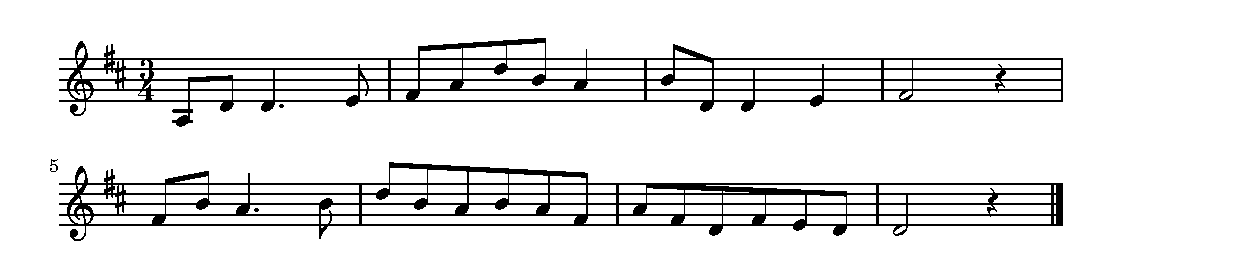
\includegraphics[clip]{akatonbo_crop.pdf}

\vspace{-10mm}

\parindent=50pt 
赤とんぼ(ゆうやけこやけのあかとんぼ)
\parindent=10pt

\vspace{10mm}


\includegraphics[clip]{amaironokami_crop.pdf}

\vspace{-10mm}

\parindent=50pt 
亜麻色の髪の乙女(あまいろのながいかみをかぜが)
\parindent=10pt

\vspace{10mm}


\includegraphics[clip]{anokowatare_crop.pdf}

\vspace{-10mm}

\parindent=50pt 
あの子はたあれ(あのこはたあれたれでしょね)
\parindent=10pt

\vspace{10mm}


\includegraphics[clip]{aogeba_crop.pdf}

\vspace{-10mm}

\parindent=50pt 
仰げば尊し(あおげばとうとしわがしのおん)
\parindent=10pt

\vspace{10mm}


\includegraphics[clip]{chouchou_crop.pdf}

\vspace{-10mm}

\parindent=50pt 
ちょうちょう(ちょうちょうちょうちょうなのはにとまれ)
\parindent=10pt

\vspace{10mm}

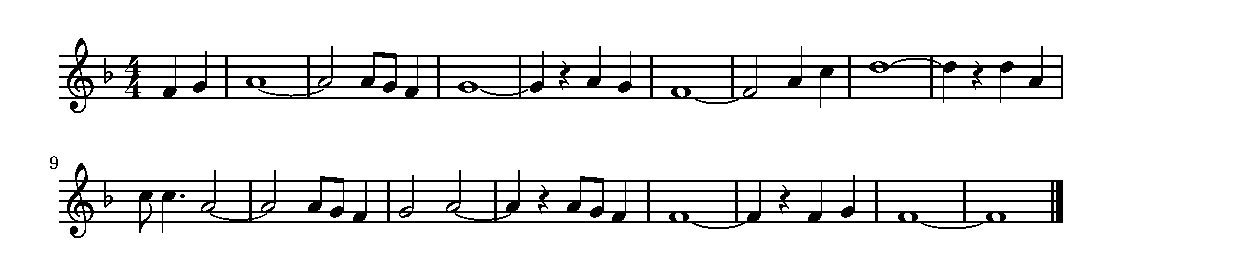
\includegraphics[clip]{countryroad_crop.pdf}

\vspace{-10mm}

\parindent=50pt 
カントリー・ロード(かんとりーろーど、このみち)
\parindent=10pt

\vspace{10mm}

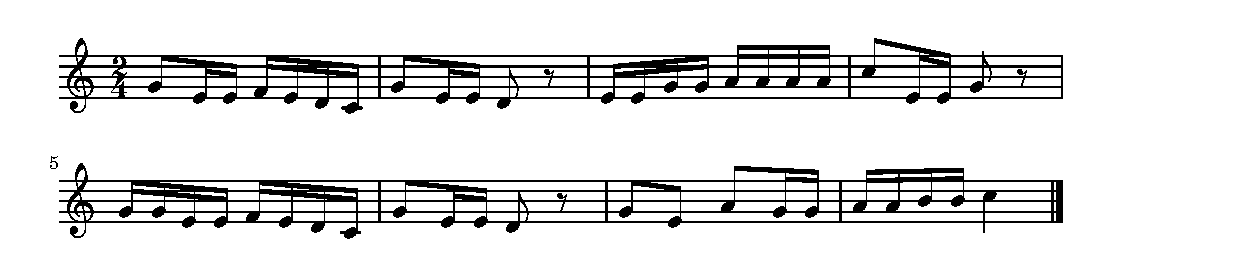
\includegraphics[clip]{donguri_crop.pdf}

\vspace{-10mm}

\parindent=50pt 
どんぐりころころ(どんぐりころころどんぶりこ)
\parindent=10pt

\vspace{10mm}


\includegraphics[clip]{fujisan_crop.pdf}

\vspace{-10mm}

\parindent=50pt 
富士山(ふじさん。あたまをくものうえにだし)
\parindent=10pt

\vspace{10mm}

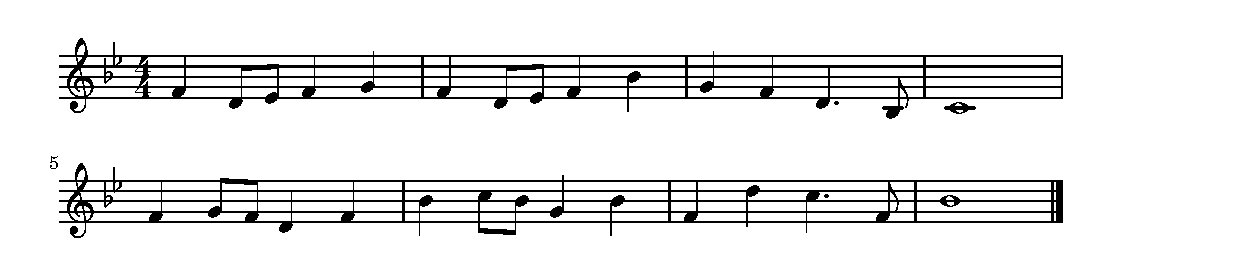
\includegraphics[clip]{harugakita_crop.pdf}

\vspace{-10mm}

\parindent=50pt 
春が来た(はるがきた)
\parindent=10pt

\vspace{10mm}


\includegraphics[clip]{harukaze_crop.pdf}

\vspace{-10mm}

\parindent=50pt 
春風(ふけそよそよふけはるかぜよ)
\parindent=10pt

\vspace{10mm}


\includegraphics[clip]{harunoogawa_crop.pdf}

\vspace{-10mm}

\parindent=50pt 
春の小川(はるのおがわはさらさらながる)
\parindent=10pt

\vspace{10mm}


\includegraphics[clip]{kawanonagare_crop.pdf}

\vspace{-10mm}

\parindent=50pt 
川の流れのように(しらずしらずあるいてきた)
\parindent=10pt

\vspace{10mm}


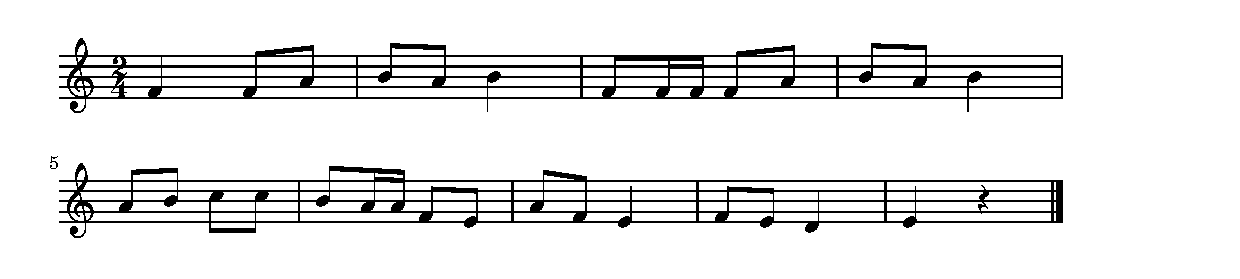
\includegraphics[clip]{usagi_crop.pdf}

\vspace{-10mm}

\parindent=50pt 
うさぎ(うさぎうさぎなにみてはねる)
\parindent=10pt

\vspace{10mm}



\includegraphics[clip]{warewaumi_crop.pdf}

\vspace{-10mm}

\parindent=50pt 
われは海の子(われはうみのこしらなみの)
\parindent=10pt

\vspace{10mm}



\includegraphics[clip]{yashinomi_crop.pdf}

\vspace{-10mm}

\parindent=50pt 
椰子の実(やしのみ。なもしらぬとおきしまより)
\parindent=10pt

\vspace{10mm}



\includegraphics[clip]{yesterdayonce_crop.pdf}

\vspace{-10mm}

\parindent=50pt 
イエスタデイ・ワンス・モア(カーペンターズ)
\parindent=10pt

\vspace{10mm}



\includegraphics[clip]{yuki100p_crop.pdf}

\vspace{-10mm}

\parindent=50pt 
勇気100パーセント(がっかりしてめそめそしてどうしたんだい)
\parindent=10pt

\vspace{10mm}



\includegraphics[clip]{yorokobi_crop.pdf}

\vspace{-10mm}

\parindent=50pt 
喜びの歌(はれたるあおぞらただようくもよ)
\parindent=10pt

\vspace{10mm}


\end{document}